the\subsection{3 февраля. Слабая сходимость}

\begin{enumerate}
    \item Определение. Естественность и полезность

    \begin{definition}
    Пусть $E$~--- нормированное пространство. Говорим, что последовательность элементов $x_n$ слабо сходится к $x$, обозн. ($x_n \weakconv x$), если \[\forall f \in E^*\; f(x_n) \to f(x).\]
    \end{definition}

    Уравнения математической физики: хотим чтобы можно было осуществлять предельный переход под знаком интеграла, поэтому нам не нужна именно равномерная сходимость, достаточно слабой сходимости.

    \item Корректность определения

    Хотим показать единственность предела.

    Предположим, что $x_n \weakconv x'$ и $x_n \weakconv x''$. По определению 

    \[ \forall f \in E^* \; f(x_n) \to f(x'), \; f(x_n) \to f(x'')\]

    По следствию~\ref{hbcorollary3} из теоремы Хана-Банаха \(x' = x''\).

    \item Слабая сходимость и сходимость по норме (сравнение)
    \begin{itemize}
        \item $\dim E$ - любая.\\
        \[\|x_n - x\| \to 0 \implies x_n \weakconv x.\]

        \begin{proof}
            \[|f(x_n)-f(x)|=|f(x_n-x)| \leqslant \|f\| \cdot \|x_n - x\| \to 0 \]
        \end{proof}
        
        \item $\dim E < \infty$
        \[\|x_n - x\| \to 0 \Leftarrow x_n \weakconv x.\]
        \begin{exercise}
            Подсказка: функционал что на $k$-ом элементе одиница а везде дальше нули. Из этого легко получить координатную сходимость а из нее следует сходимость по норме. (Шамаров доказывал, TODO переписать)
        \end{exercise}
        \item $\dim E = \infty$
        \[\|x_n - x\| \to 0 \not\Leftarrow x_n \weakconv x.\]

        \begin{counterexample} $H = l_2(\R), e^n = (0, \ldots, 0, 1, 0 \ldots)$. Понятно, что сходимости по норме нет. Однако, если рассмотреть определение и перейти к скалярному произведению:
        \[ \angles{e^n, y} = y_n \to 0 = \angles{0, y}.\]
        Причем \(y_n\) стремится к нулю как член сходящегося ряда.

        Откуда получаем, что $e^n \weakconv 0$.
        \end{counterexample}

        \begin{exercise}
            В $l_2$ секвенциально слабое замыкание $\overline{S(0, 1)} = \overline{B}(0, 1)$
        \end{exercise}
    \end{itemize}

    \item Слабая сходимость в гильбертовом пространстве

    Пусть $H$ ~--- гильбертово пространство. По теореме~\nameref{Riss-Freshe} $f(x)=\angles{x, y},\; y \in H$. Тогда $f(x_n) \to f(x) \Leftrightarrow \angles{x_n, y} \to \angles{ x, y }$.

    Можно ли придумать норму, которая порождает эту сходимость? \textbf{Нет, нельзя, это нетривиальный факт}.

    \item Слабая сходимость и выпуклость

    \begin{exercise}
        \begin{enumerate}[label=\alph*)]
            \item В гильбертовом пространстве
            \[
            \|x_n\| \leqslant 1, x_n  \weakconv x \implies \|x\| \leqslant 1
            \]

            \item В произвольном пространстве это тоже выполнено
            
           \begin{proof}
            \[\forall f \in E^* \ |f(x_n)| \to |f(x)| \leqslant 
            \|f\| \cdot \underbrace{\|x_n\|}_{\leqslant 1} \implies |f(x)| \leqslant \|f\|\]

            По следствию~\ref{hbcorollary4} из теоремы Хана-Банаха 
            $\|x\| = \sup_{\|f\| = 1} |f(x)| \leqslant 1$.
            \end{proof}
        \end{enumerate}
        
    \end{exercise}

    Возьмём в нормированном пространстве $E$ произвольное замкнутое выпуклое тело $S$ и $S \ni x_n \weakconv x$. Верно ли, что $x \in S$? \textbf{Ответ да: теорема Мазура 1933 год.}

    \item В гильбертовом пространстве $\| x_n - x \| \to 0 \Rightarrow x_n \weakconv x.$
    
    Можно ли к слабой сходимости добавить условие, чтобы обе части были равносильны?
    В гильбертовом пространстве можно, достаточно чтобы $\|x_n\| \to \|x\|$. Это какой-то номер задания.

    \item Слабая топология и слабая сходимость

    Можно придумать топологию, порождающую слабую сходимость, но мы об этом не говорим. Рассмотрим разные виды замыканий:
    \[\overline{S(0; 1)} \subset \overline{S(0; 1)}^{\text{ секв. сл.}} \subset \overline{S(0; 1)}^{\text{ сл.}}\]

    Чем слабее топология, тем больше замыкание. Чем сильнее топология, тем проще отображению быть непрерывным.

    \underline{Запас непрерывности у ограниченных линейных операторов}
    
    Рассмотрим $E$ и класс линейных ограниченных отображений 
    $\mathcal{L}(E)$. $A \in \mathcal{L}(E)$~--- непрерыно по норме $\| \cdot \|$. А в слабой топологии? Просто по определению и следствиям останется непрерывным.
    \begin{theorem}[7.2]  % нумерация лектора
        Пусть $E_1, E_2$~--- нормированные пространства, $A \in \mathcal{L}(E_1, E_2)$. Тогда из условия $x_n \weakconv x$ следует, что $Ax_n \weakconv Ax$.
    \end{theorem}
    \begin{proof}\textit{ Cогревающее душу.}\\
    \begin{figure}[H]
            \centering
            
\includegraphics[width=0.4\textwidth]{images/7_2.jpg}
    \end{figure}
    Пусть есть оператор $A:\;E_1 \to E_2$. Возьмем произвольный функционал $g \in E_2^*$. Рассмотрим отображение $f = g \circ A$~--- линейный непрерывный функционал. Тогда $f \in E_1^*$.

    Получаем, что по определению слабой сходимости
    \[\forall g \in E_2^* \; gA(x_n) \to gA(x)  \implies g(Ax_n) \to g(Ax) \implies  A x_n \weakconv Ax.\]
    \end{proof}

    \textbf{Изометрия} $E$ и $E^{**}$: $\pi: E \to E^{**}$. $\pi x = F_x \in E^{**}, F_x(f) = f(x)$.
    \begin{figure}[H]
            \centering
            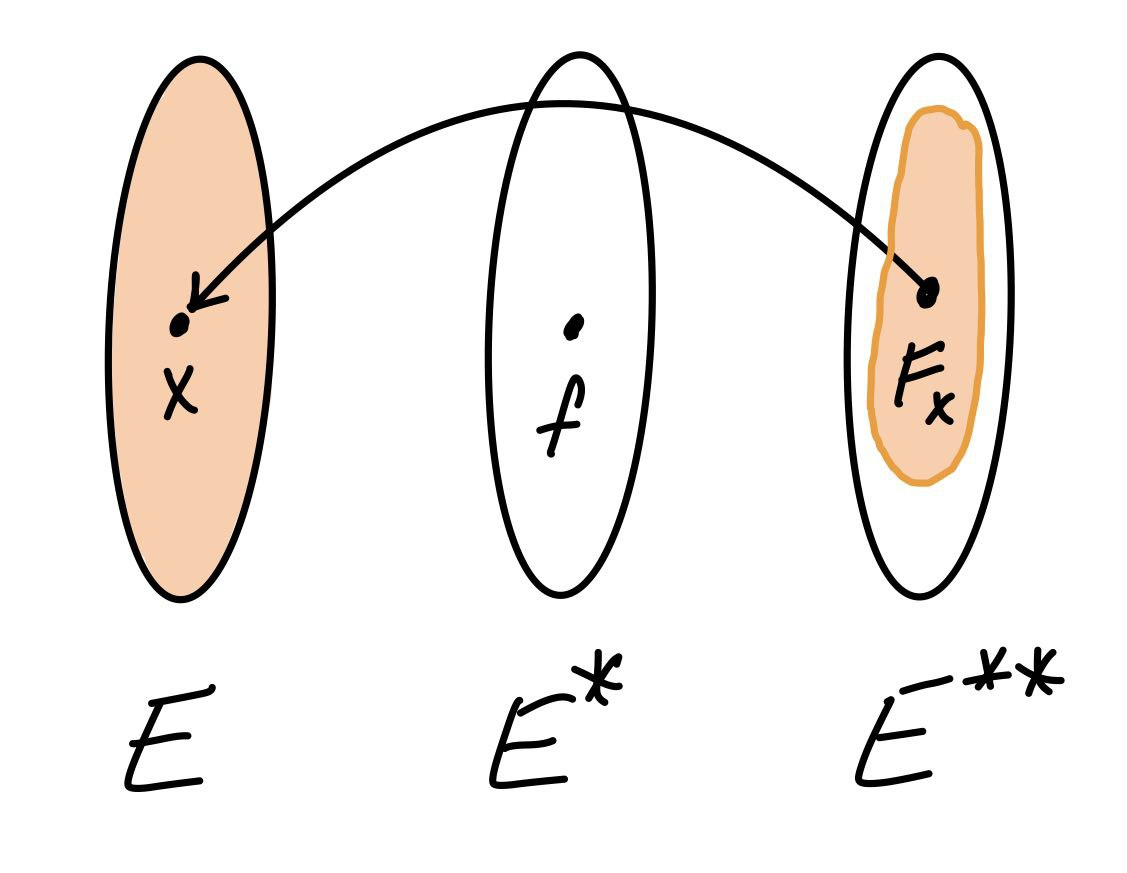
\includegraphics[width=0.4\textwidth]{images/isometry.jpg}
    \end{figure}
    В силу следствия~\ref{hbcorollary4} из теоремы Хана-Банаха

    \[ \| F_x \| = \sup_{\|f\|=1} |F_x(f)|=\sup_{\| f \| = 1} |f(x)|=||x|| \]

    \begin{note}
    \[x_n \weakconv x \Longleftrightarrow \forall f \ f(x_n) \to f(x) \Longleftrightarrow F_{x_n}(f) \to F_x(f) \; \forall f\]
    Это означает поточечную сходимость $F_{x_n}$ к $F_x$.
    \end{note}
    
    \item Воспоминания следствия теоремы Банаха-Штейнгауза:~\nameref{bshetengcorollary}.
    У нас операторы $F_x: E^* \to \K$. Помним что так как $\K$~--- полное, $\mathcal{L}(E, \K)$~--- полное.

    \begin{theorem}[7.1]\label{thm7_1}
        Пусть $E$~--- ЛНП. Тогда последователность $x_n \in E,\; x_n \weakconv x$ тогда и только тогда когда выполнено:\\
        \[\begin{cases}
        \text{1) последовательность $\{\|x_n\|\}$~--- ограничена}\\
        \text{2) $\forall s \in S \subset E^*: [S] = E^*,\;\; f(x_n) \to f(x )$}\\
        \end{cases}\]
    \end{theorem}

    \begin{exercise}[10-8]
    Непрерывность скалярного произведения:

    \[x_n \to x, y_n \to y \implies \angles{x_n, y_n} \to \angles{x, y}\]

    При слабой сходимости это уже не работает. Пример: $\angles{e^n, e^n}=1 \not\to 0$

    Если сделать только одну сходимость слабой, то непрерывность все еще сохраняется
    \end{exercise}
\end{enumerate}